\documentclass[a4paper]{article}
\usepackage{CJKutf8, geometry, graphicx, hyperref, xcolor, listings}
\geometry{margin=4cm}

% Python for external files
\newcommand\pythonexternal[2][]{{
\pythonstyle
\lstinputlisting[#1]{#2}}}

\title{\textbf{中間人攻擊}}
\author{B073040047 楊志璿 \and M093040096 李天朗 \and M093040094 王文濤}

\begin{document}
\begin{CJK*}{UTF8}{bsmi}
    \maketitle
    \newpage

    \tableofcontents
    \newpage

    \section{摘要}
    這是一篇關於中間人攻擊的期末報告,題目要求必須要實做 \ HTTPS 連線之竊取帳號密碼。
    本篇報告介紹本期末專案的: HTTPS 中間人攻擊、即時密碼測錄、實做成果與中山大學網路大學之
    登入安全探討。\\

    本專案開放原始碼於:\url{https://github.com/25077667/Man-in-the-Middle-Attack}
    \newpage

    \section{本文}
    建議具有中間人攻擊之相關背景知識,再來閱讀此篇報告。關於中間人攻擊之相關內容,礙於篇幅,本文將不再贅述。\\
    藉由無知使用者,在不檢查憑證之情況下,實現隱形中間人攻擊。
    \subsection{架構}
    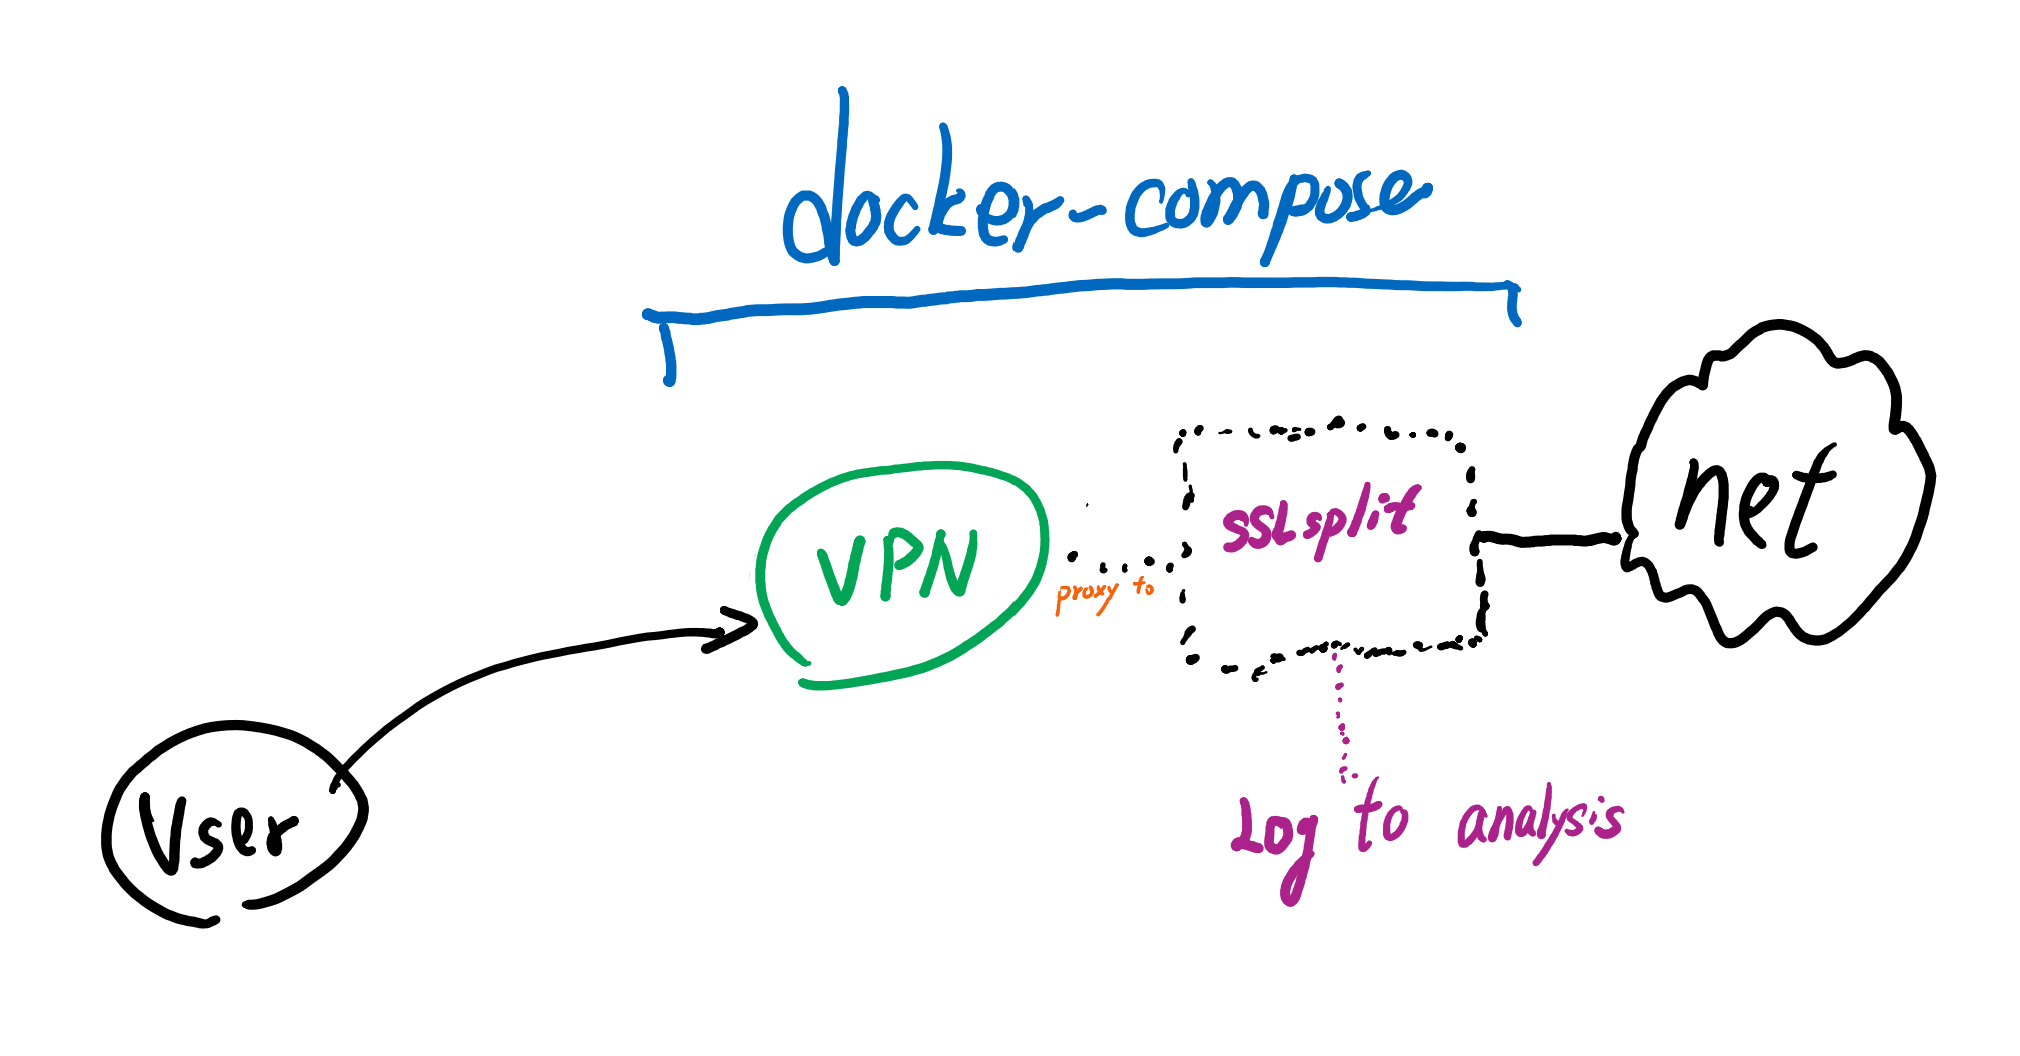
\includegraphics[width=\textwidth]{images/image_2022-01-14_01-52-22.png}
    docker-compose 部份,僅用於「重現」方便,沒有限制必須使用\ docker 相關技術。\\

    在使用者連上\ VPN 之情況下,可以使用\ iptables 於 VPN 後端,將\ VPN 所接收之資料,交給
    \ sslsplit 代理轉發。實際上,使用者是無法知道\ sslslpit 之存在的,因為\ VPN 本身即是一
    種代理 (proxy)。

    \subsection{攻擊情境}
    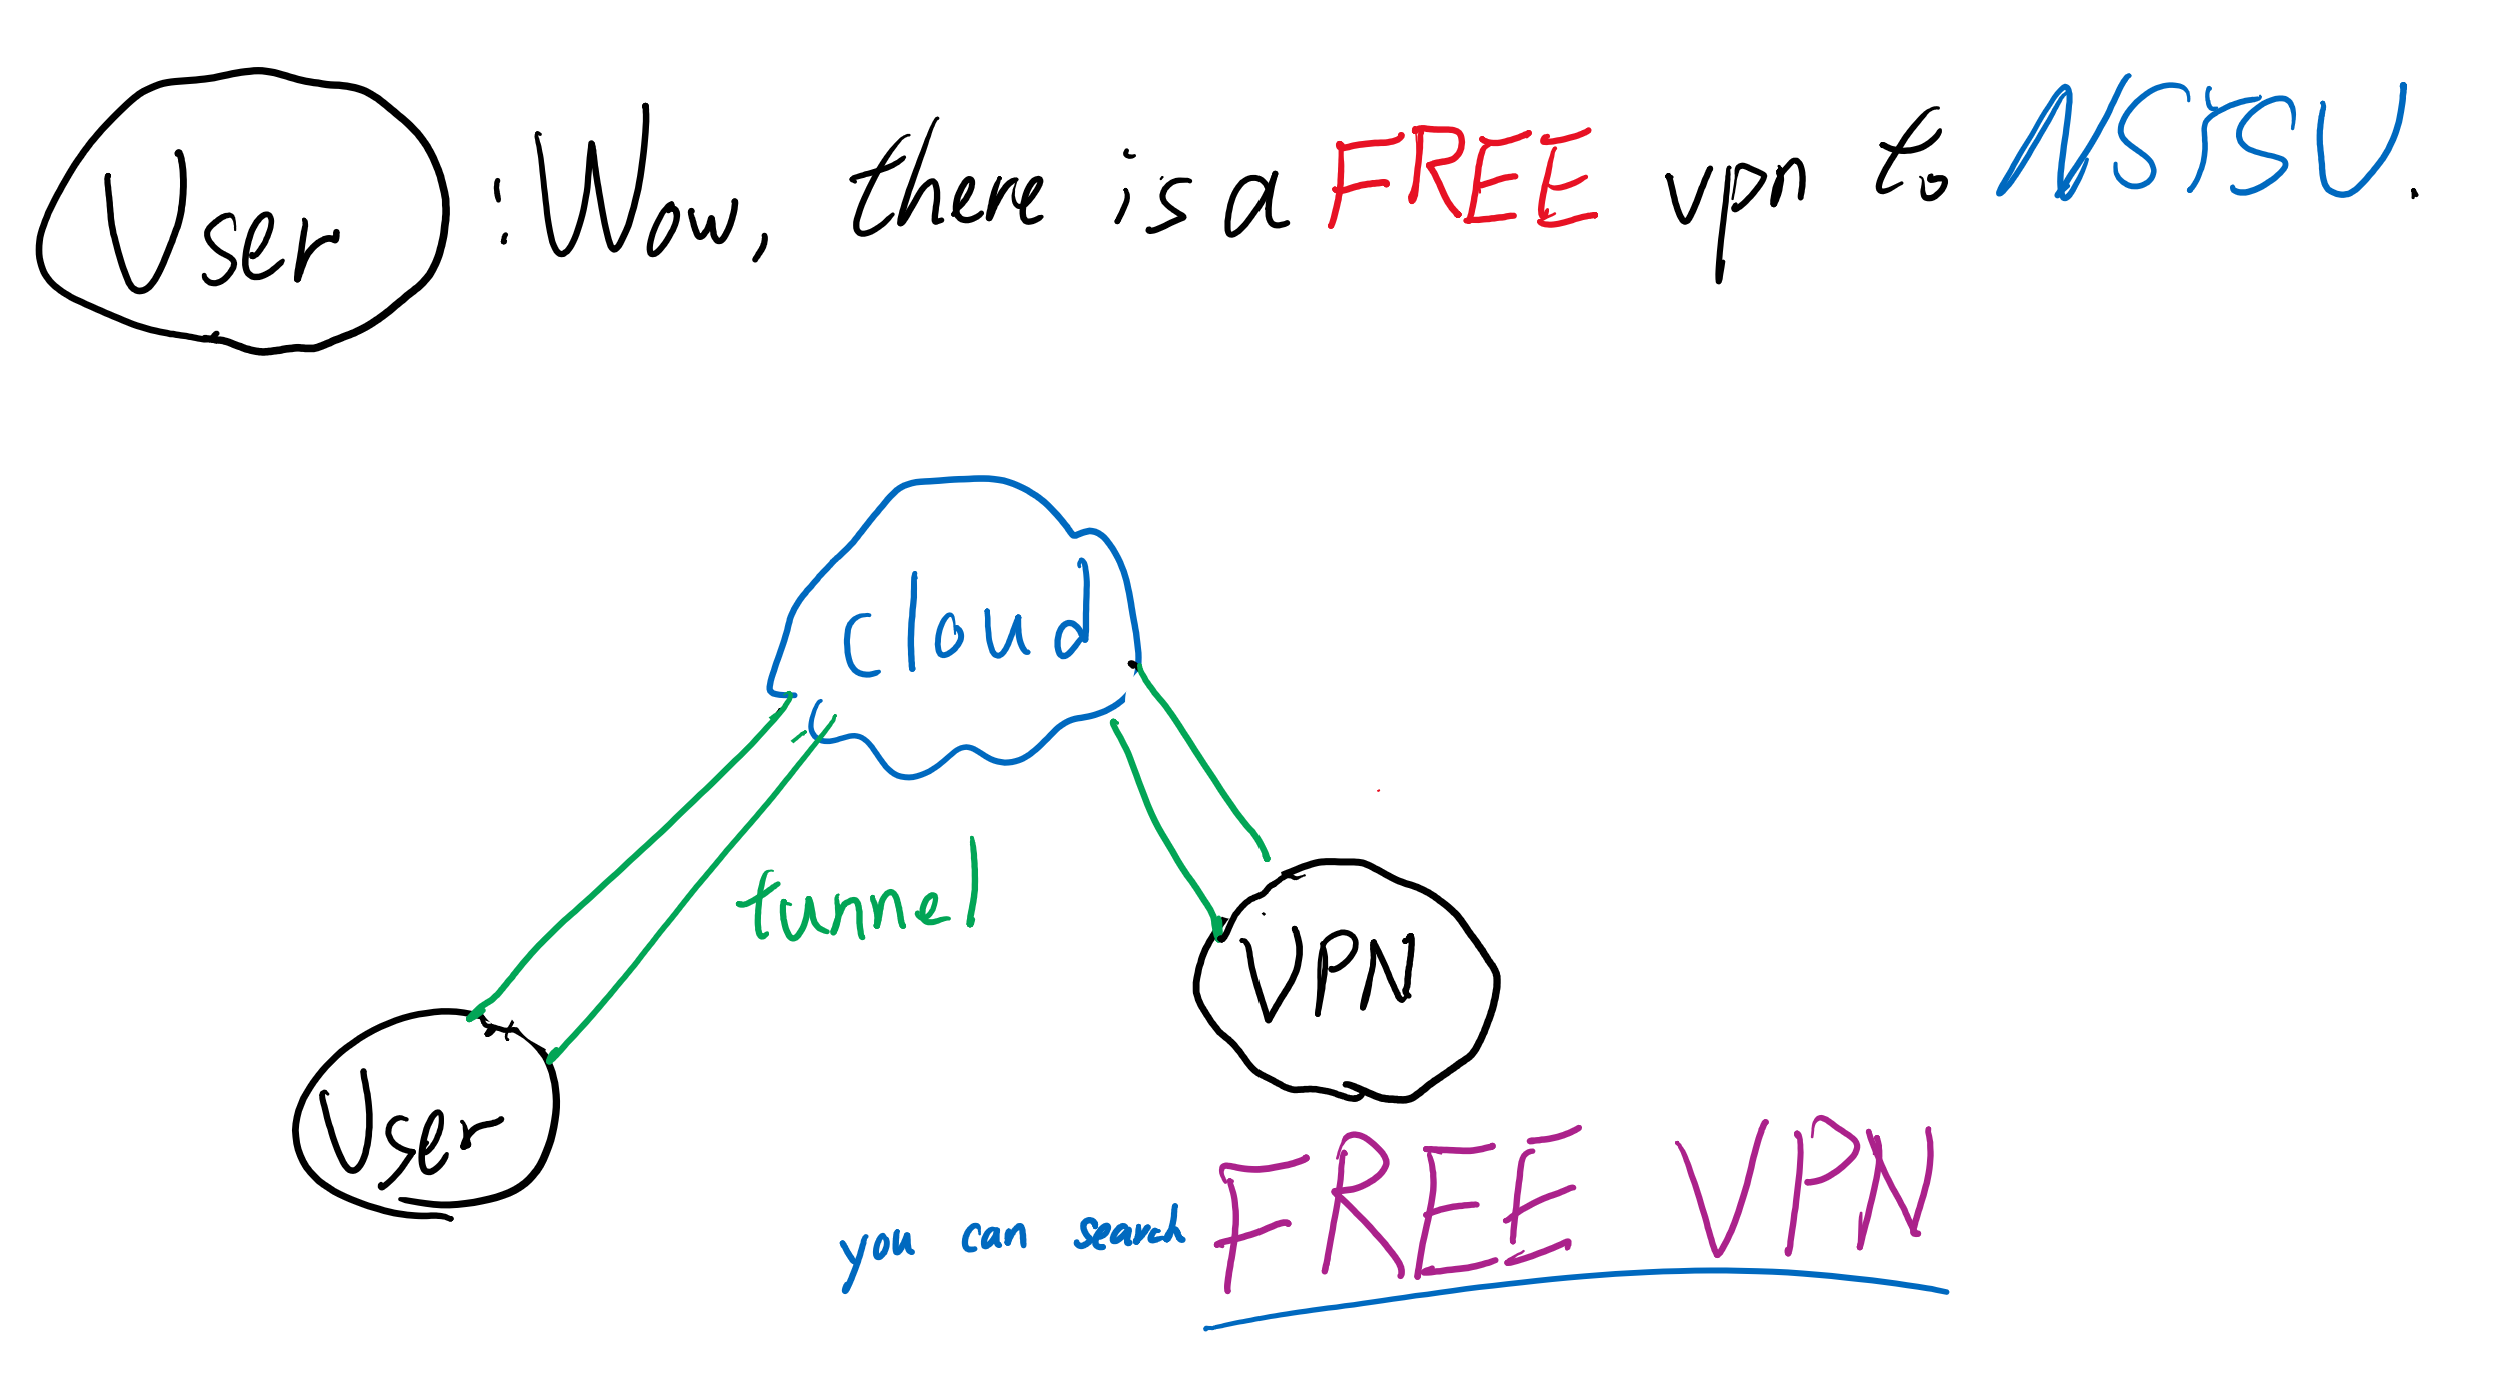
\includegraphics[width=\textwidth]{images/image_2022-01-14_01-42-43.png}\\

    使用者想要使用免費之中山大學學術網路服務,中山大學之\ ip 有付費訂閱許多期刊,以利學術研究。
    於是使用者發現有一個不用中山大學學生證的「免費」\ VPN 即可以使用中山大學之\ ip,於是使用
    者便直接陷入本次實驗之中間人攻擊陷阱。\\

    有此一說\footnote{\url{https://games.yahoo.com.tw/meme-111554483.html}}
    :「我需要網址,為了學術研究」。\\
    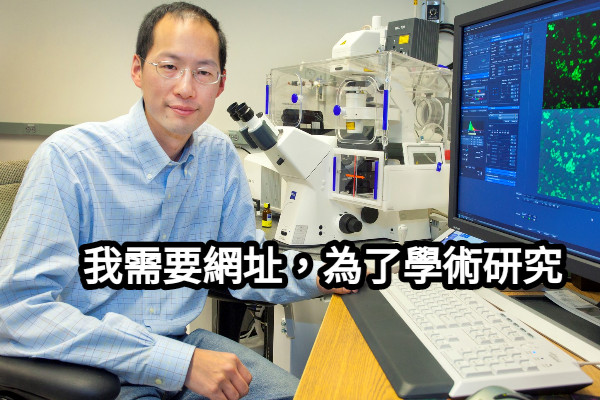
\includegraphics[width=\textwidth]{images/1613538663684.jpg}
    因此本專案作為學術用途,連線上中山大學之學術網路,以利學術研究。
    或者可以支持「開放學術資源\footnote{\url{https://en.wikipedia.org/wiki/Open_access}}」、
    「開放知識運動\footnote{\url{https://en.wikipedia.org/wiki/Access_to_Knowledge_movement}}
    \footnote{\url{https://tw.okfn.org/}}」,學術知識為全人類所共有,並非少數研究機構所
    把持。

    \subsection{即時檢視受害者資訊與實做}
    本篇研究報告,提出此機制可以即時檢視受害者資訊,而不用處理事後\ pcap 封包紀錄擋。因為通常網路流量都相當大,
    將所有封包資訊儲存並分析,是不切實際的作法。\\

    sslsplit\footnote{\url{https://www.roe.ch/SSLsplit}} 攻擊工具會一個輸出目錄,
    將其經過之流量,解密後輸出至指定目錄檔案。
    我們可以透過 \ tmpfs 映射一塊記憶體空間,並且掛載(mount)於給定目標(例如 \underline{/data}
    );並且由駭客所撰寫背景程式監聽\footnote{\url{https://man7.org/linux/man-pages/man7/inotify.7.html}}
    此記憶體空間之檔案關閉事件,進而送出該檔案給語法解析器(parser)解析封包內容。\\

    此機制之完整實做並未出現在期末上台報告中,因為正當我們測試本校網路大學時\  HTTPS 加密連線,我們應該將
    上台報告改變為如下 \ref{cu} 之弱點分析。但是,此機制將在此以圖例與 \ Python 程式碼呈現。另外我們可以用\
    docker-compose 保證\ {\color{red} Hacker} container "create" before {\color{green} VPN} container.
    \newpage

    Docker-compose 架構圖:\\
    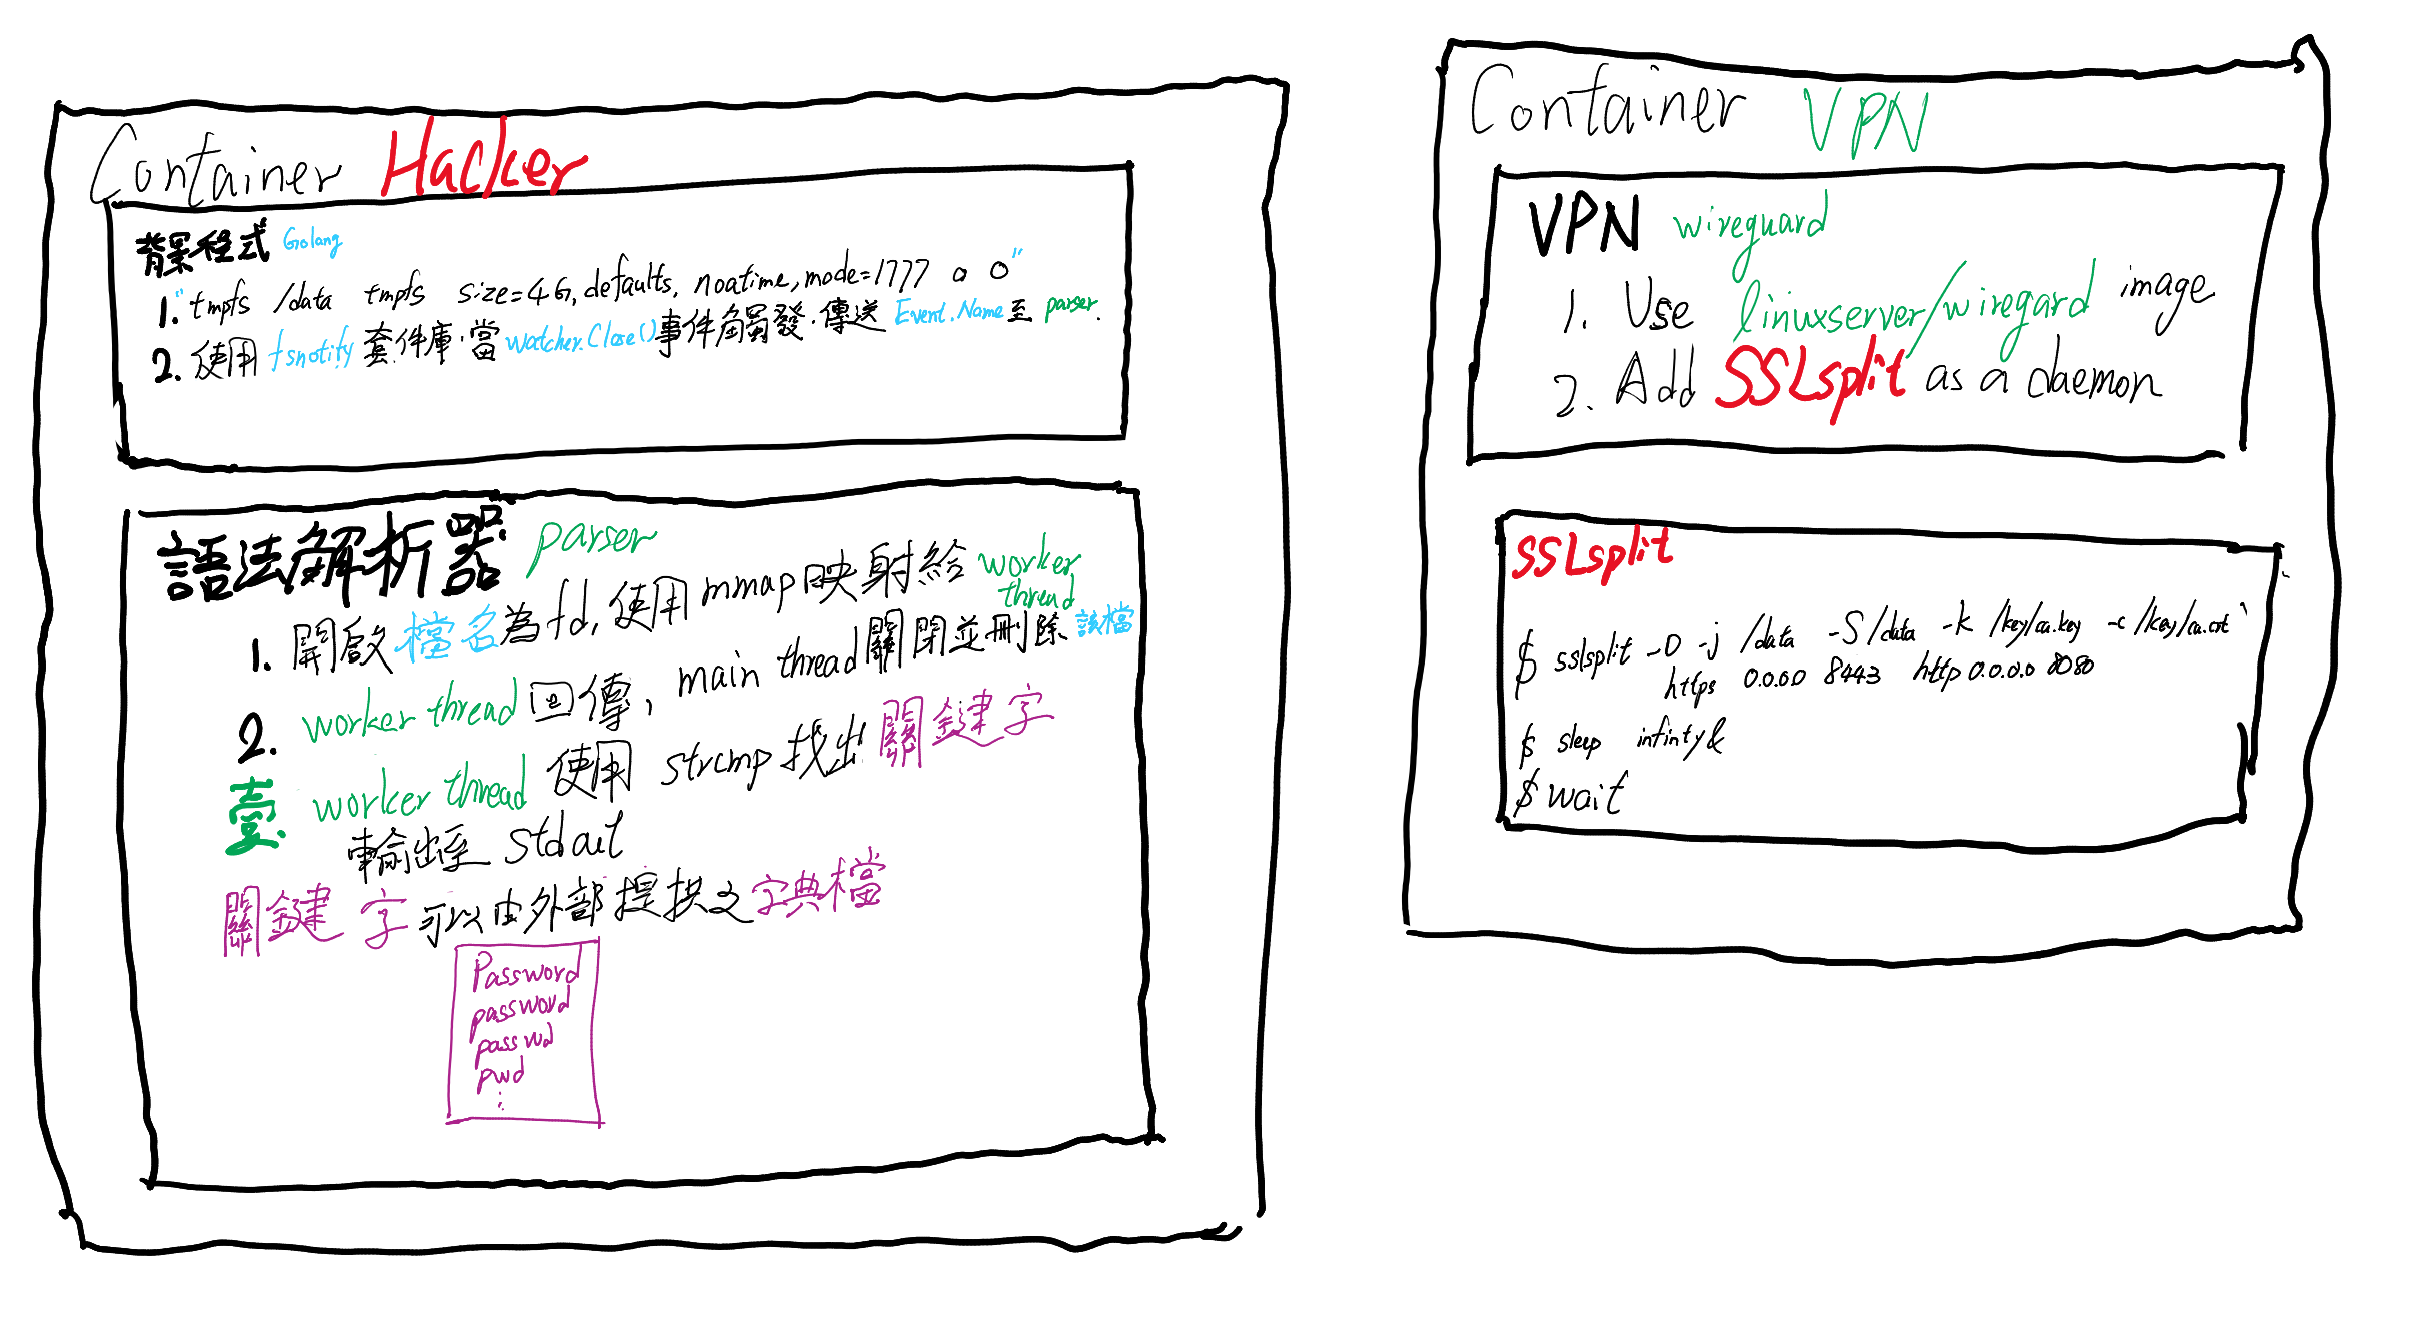
\includegraphics[width=\textwidth]{images/image_2022-01-18_17-58-35.png}\\
    解析 \ HTTP Response 之 Python 範例
    \lstinputlisting[language=Python]{src/main.py}
    \newpage

    \subsection{防禦方式}
    \begin{itemize}
        \item 檢查憑證
        \item 憑證固定
        \item 網路治理
    \end{itemize}

    \section{成果}
    受害者登入界面:\\
    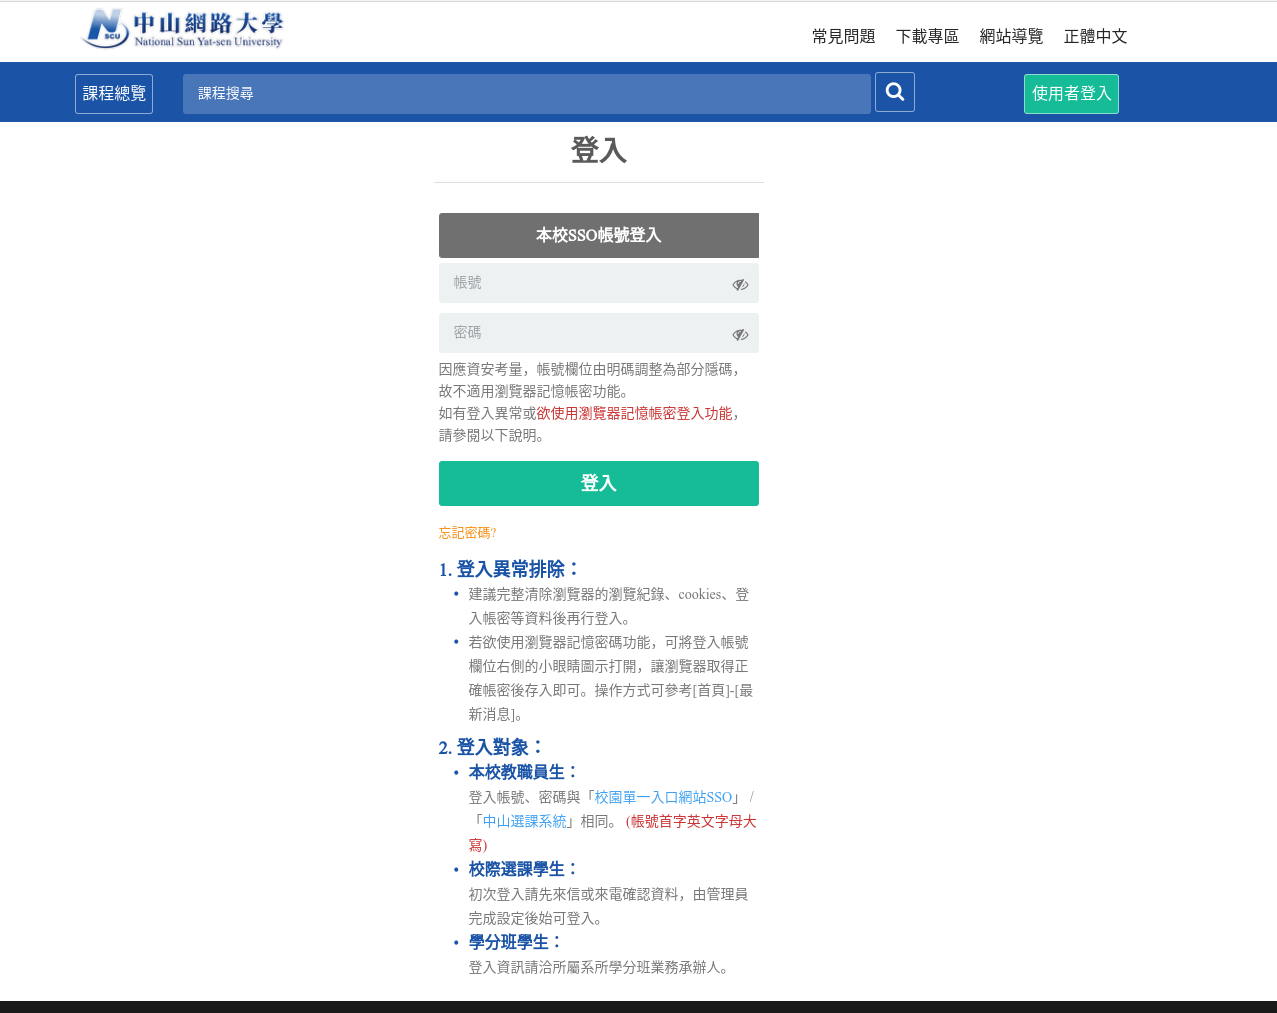
\includegraphics[width=\textwidth]{images/Screenshot_2022-01-18_18-31-30.png}
    \newpage
    受害者成功登入:\\
    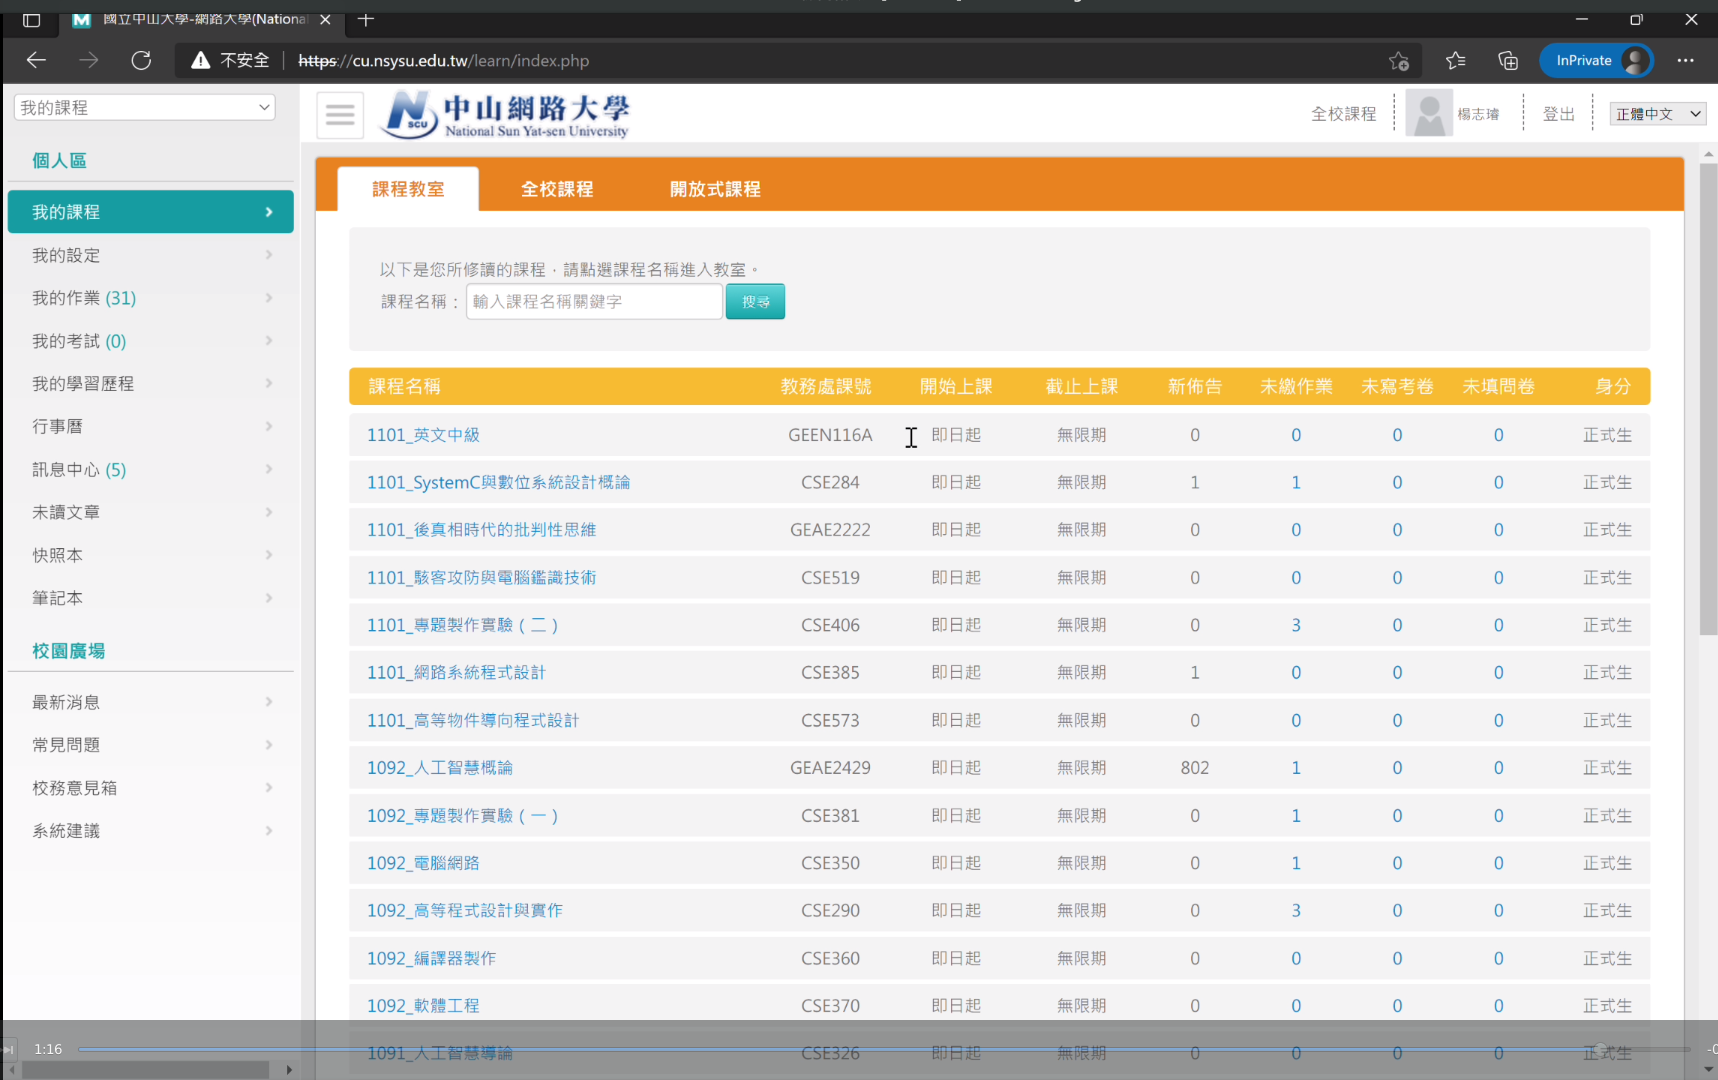
\includegraphics[width=\textwidth]{images/Screenshot_2022-01-18_18-24-27.png}\\
    中間人擷取到 POST 之隱私資料:\\
    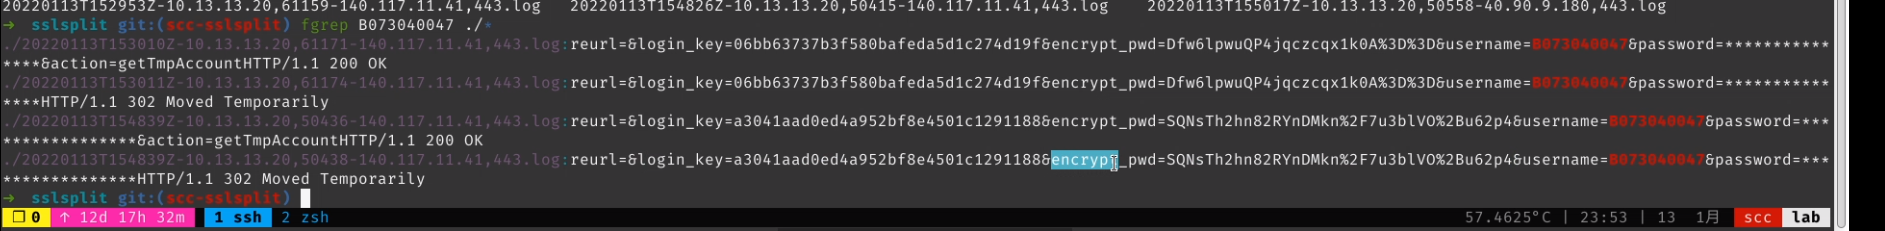
\includegraphics[width=\textwidth]{images/Screenshot_2022-01-18_18-28-12.png}
    \label{data_mid}

    \subsection{國立中山大學網路大學之弱點分析}
    \label{cu}
    從上 \ref{data_mid} 圖可見密碼欄位全為 `*' 符號,我們猜測中山網路大學可能有考量到中間人攻擊的
    可能性,但是仔細觀察\ login\_key 與\ encrypt\_pwd 可以發現其中端倪。
    根據多年駭客經驗,該欄位是 base64 編碼(encode)。因此翻閱網路大學\ base64 編碼\ encrypt\_pwd
    處可以發現:\\
    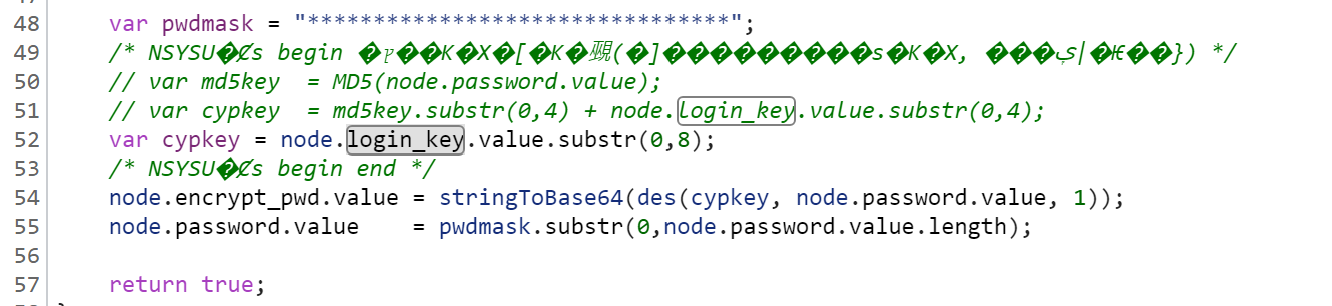
\includegraphics[width=\textwidth]{images/image_2022-01-14_01-02-16.png}\\
    發現加密方式如程式碼,為\ DES 加密。此加密為已知弱「對稱式加密」,因此我們可以根據\ DES 演算法,
    推導出此加密反函數,並且擁有該加密金鑰\ login\_key 鑲嵌於網頁原始碼中:\\
    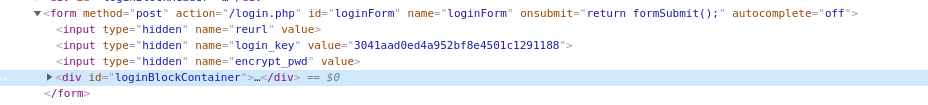
\includegraphics[width=\textwidth]{images/Screenshot_2022-01-14_01-11-36.png}\\

    因此,此防禦對於\ APT 攻擊\textbf{完全無效},當駭客有實際如此觀察過網路大學之實做,完全可以透過\ DES 反
    函數解密出受害者密碼。造成「無謂的加密」問題。

    \section{結論}
    本專案之中間人攻擊箬搭配\ DNS 污染,於\ VPN 端,使用者可以在完全沒看到「網頁不安全」之警示訊息於瀏覽器
    ,但是實際上已經被中間人攻擊。唯一的檢查方式就是打開憑證資訊,確認此憑證是由權威的受信任的數字證書認證機構
    頒發。\\

    否則,現行網路無法發覺您是否正在被中間人攻擊當中。

    \subsection{貢獻比例}
    \begin{center}
        \begin{tabular}{||c c||}
            \hline
            姓名   & 貢獻比例 \\ [0.5ex]
            \hline\hline
            楊志璿 & 100\%    \\
            \hline
            李天朗 & 0\%      \\
            \hline
            王文濤 & 0\%      \\
            \hline
        \end{tabular}
    \end{center}
    
\includegraphics[width=\textwidth]{images/Screenshot_2022-01-18_15-09-06.png}
    \newpage

    這是第 10 頁
    \newpage
    這是第 11 頁
    \newpage
    這是第 12 頁
    \newpage
    書面報告結束
    \newpage

\end{CJK*}
\end{document}